% Format: max 3 pages excluding references, single column.
% Every paper, dataset, library and model used must be in refs.bib AND cited in the text.
\documentclass[11pt]{article}

\usepackage[margin=1in]{geometry}
\usepackage[T1]{fontenc}
\usepackage[utf8]{inputenc}
\usepackage{lmodern}
\usepackage{amsmath}
\usepackage{booktabs}
\usepackage{graphicx}
\usepackage{enumitem}
\usepackage[numbers,sort&compress]{natbib}
\usepackage[hidelinks]{hyperref}
\usepackage{xurl}

\setlist{nosep,leftmargin=*}
\setlength{\parskip}{0.4em}
\setlength{\parindent}{0pt}

\title{\vspace{-2.2em}\textbf{DGA Classifier from Domain Names:\\Family-First or Direct Binary?}}
\author{
  Roudy Barakat \quad \texttt{rtb07@mail.aub.edu} \\
  Abdo Sebailli \quad \texttt{ams86@mail.aub.edu} \\[0.3em]
  \small American University of Beirut
}
\date{\vspace{-1.5em}}

\begin{document}
\maketitle

\section{Problem and Motivation}
Malware uses Domain Generation Algorithms (DGAs) to generate many domains from a
shared seed, so infected hosts can reach the attacker without a hard-coded
address that defenders could block~\cite{plohmann2016dgarchive}. Real detection
also uses network signals such as the NXDOMAIN rate and query
periodicity~\cite{antonakakis2012pleiades}; this project focuses on detecting
DGAs from the domain name alone. The difficulty is that ``DGA'' is not one
pattern: some families produce random strings (\texttt{gqspwpsurdun.ru},
CryptoLocker) or hex hashes (\texttt{2c3f1e3326cca35b757ec704b2413a30.org},
Bamital), while others join dictionary words (\texttt{kneemanualgirl.com},
\texttt{whetherspread.net}) and look much closer to legitimate names.

\textbf{Question.} When the final decision is DGA vs.\ legitimate, should a
classifier first learn the individual DGA families (each family + legitimate,
with the prediction collapsed to DGA/legitimate) or learn DGA vs.\ legitimate
directly?

\textbf{Why it matters.} The answer is for teams that build name-based DGA
filters, for example in DNS resolvers or security products, where a model must
judge a single query before any connection is made. If family-first training
wins, family labels are worth collecting even when only a binary decision is
needed, and simpler models may become accurate enough to deploy. If it does
not, the simpler binary setup is enough.

\textbf{Goal.} For each model we evaluate, measure the difference in macro-F1 on
the DGA/legitimate decision between family-first and direct binary training, on
the same test set and averaged over 5 random seeds. We count family-first as
better when its mean macro-F1 is higher by more than the standard deviation
across seeds.

\section{Impact}
\textbf{If it succeeds.} Teams that build name-based DGA filters get a clear
rule for how to train them: if family-first wins, it is worth collecting and
maintaining family labels even when only a DGA/legitimate verdict is shipped;
if both setups tie, the cheaper binary labels are enough. The per-family results
also show which kinds of DGA (random-string or dictionary-based) a name-only
detector can and cannot catch, which tells analysts where to expect blind spots.

\textbf{If it fails.} If neither setup separates some families from legitimate
domains, in particular dictionary-based ones, that is evidence that the name
alone does not carry enough signal for them. Detection would then need network
traffic features, such as the NXDOMAIN rate, the periodicity of queries, and how
many distinct, previously unseen domains a single host
queries~\cite{antonakakis2012pleiades}. Knowing which families need these
signals is itself a useful result.

\textbf{Risks of using the result.}
\begin{itemize}
  \item \emph{Errors do not cost the same.} A missed DGA domain (false negative)
  leaves an infected host talking to its attacker. A legitimate domain flagged
  as DGA (false positive) blocks a real service and adds to alert fatigue. Since
  almost all real DNS traffic is legitimate, even a small false-positive rate
  produces many false alarms.
  \item \emph{Bias in the data.} Legitimate examples come from a popularity
  ranking (Tranco~\cite{lepochat2019tranco}), which over-represents popular
  sites. Legitimate but unusual names, such as non-English, short or
  machine-generated CDN hostnames, may be flagged unfairly. Families with fewer
  than 300 known domains are left out of our data, so our results say nothing
  about them.
  \item \emph{Limited validity.} We test only families seen in training.
  Attackers can change their algorithms, so results do not guarantee detection
  of new or adversarial DGAs.
\end{itemize}

\section{Related Work}
\citet{woodbridge2016lstm} introduced deep learning for DGA detection with a
character-level LSTM trained on Alexa domains and 30 DGA families. They built a
binary model and a separate family model: the binary model reached an AUC of
0.9993, but the family model's macro-F1 was only 0.54, rising to 0.96 when
similar families were grouped. We adopt macro-F1, and their grouping result
suggests that the labels matter. They never collapsed the family model back into
a DGA/legitimate detector, which is the comparison we make.

\citet{gregorio2024incremental} classified 61 DGArchive families with a
character-level CNN, reaching an average F1 of 84\%, with some families at 0\%.
Their model has no legitimate class, so it cannot be used as a detector. We reuse
this CNN, add the legitimate class, and test whether confusions between DGA
families still matter once predictions are collapsed to DGA/legitimate.

\citet{torrealba2025deepdga} proposed DeepDGA, which combines a character-level
BiLSTM with word embeddings for binary detection on 25 families. It exceeds 0.97
precision on dictionary-based DGAs, where feature-based models stay below 0.89.
We take dictionary DGAs as the hardest case and report them separately. They
close that gap with a bigger architecture; we test whether richer labels help
simpler models.

\citet{shahzad2021dga} compared LSTM, BiLSTM and GRU for binary detection on
over two million domains. The LSTM reached 87\% accuracy and an AUC of about
0.98, with little difference between the three. We follow their preprocessing
(removing duplicates after stripping the TLD) and their 80/10/10
train/validation/test split. Since changing the architecture barely mattered, we
change the training labels instead, and report per-family results, which they do
not.

\citet{dahal2019autoencoded} compressed character-count vectors with an
autoencoder and classified them with a neural network or an SVM on 11 DGA
families. They reached 88\% accuracy, which fell to 78\% on families not seen in
training. We use character counts, as they do, as a simple input for our
baseline. They target unseen families, while we focus on known ones; their drop
shows the limit of our stratified split.

\section{Data}
\textbf{Sources.}
\begin{itemize}
  \item \emph{DGA:} Greg{\'o}rio and Cansian, Mendeley Data v1, 2025, CC~BY~4.0,
  \url{https://data.mendeley.com/datasets/nhvyvytn2h/1}~\cite{gregorio2025dataset}:
  3{,}090{,}661 domains in 160 families, from DGArchive~\cite{plohmann2016dgarchive}
  (Sep--Oct 2025).
  \item \emph{DGA:} C.~Givre, Kaggle ``DGA dataset'' v1, 2021, license not stated
  (academic use), \url{https://www.kaggle.com/datasets/gtkcyber/dga-dataset}~\cite{givre2021kaggle}:
  80{,}000 domains in 7 families.
  \item \emph{Legitimate:} Tranco top 1M~\cite{lepochat2019tranco}, list
  \texttt{64VVX} (17~Sep--16~Oct 2026), \url{https://tranco-list.eu/list/64VVX}.
  The legitimate rows of the two DGA datasets are not used.
\end{itemize}

\textbf{Size, input and target.} 1{,}999{,}335 domains: 999{,}664 legitimate and
999{,}671 DGA in 103 families (Fig.~\ref{fig:data}, Table~\ref{tab:stats}). The
input is the full domain name, TLD included (4--93 characters); all features are
derived from it. The targets are the binary label and the family (\texttt{legit}
or one of 103). We use pandas~\cite{mckinney2010pandas} and
Matplotlib~\cite{hunter2007matplotlib}.

\begin{figure}[h]
  \centering
  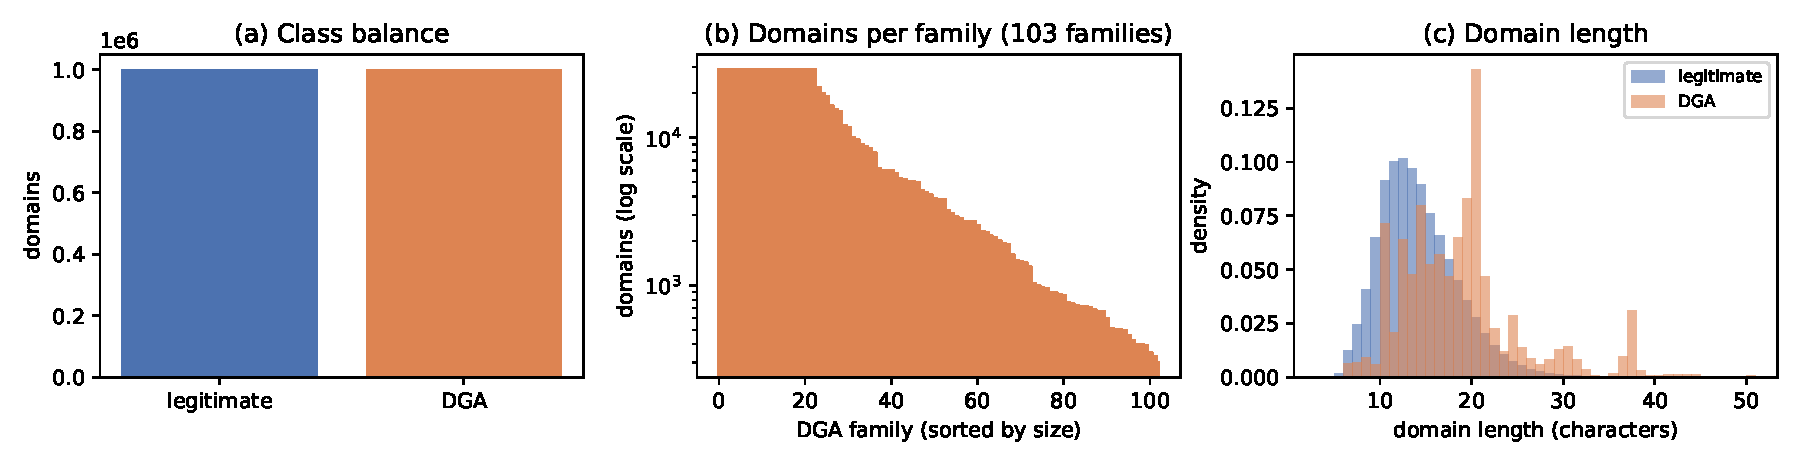
\includegraphics[width=\linewidth]{figures/data_overview.pdf}
  \vspace{-1.8em}
  \caption{(a) Class sizes; (b) domains per DGA family (log scale); (c) domain length.}
  \label{fig:data}
\end{figure}

\begin{table}[h]
  \centering
  \footnotesize
  \setlength{\tabcolsep}{4pt}
  \caption{Statistics per class. Entropy (bits) and digit ratio are computed on
  the part before the TLD.}
  \label{tab:stats}
  \begin{tabular}{lrrrrrrl}
    \toprule
    Class & Domains & Families & Mean length & Entropy & Digit ratio & TLDs & Top TLD \\
    \midrule
    Legitimate & 999{,}664 & --  & 13.7 & 2.79 & 0.038 & 1{,}030 & .com (42\%) \\
    DGA        & 999{,}671 & 103 & 18.4 & 3.17 & 0.149 & 273     & .com (23\%) \\
    \bottomrule
  \end{tabular}
\end{table}

\textbf{Cleaning.} There are no missing values. We drop 330 domains found in both
Tranco and a DGA list (e.g.\ \texttt{pywolwnvd.biz}, family \texttt{m0yv}), 141
duplicates and 7 invalid strings. Kaggle family names are mapped to Mendeley names
by domain shape (e.g.\ \texttt{newgoz} $\rightarrow$ \texttt{gameover}).

\textbf{Balancing.} After cleaning, the 161 DGA families range from 2 to 519{,}280
domains. We keep all legitimate domains, merge the 59 families with fewer than 300
domains into \texttt{other\_dga}, and cap each family at 29{,}120 domains so that
DGA and legitimate are equal in number. Sample weights give legitimate and DGA half
each and, within DGA, are proportional to $1/\sqrt{n_f}$ ($n_f$: family size), so
no family weighs more than 9.9 times another. The data are split 80/10/10
(train/validation/test), stratified by family.

\textbf{Biases.} Tranco favours popular sites. DGA families use few TLDs (23 use
only one, vs.\ 1{,}030 TLDs for legitimate domains), so the TLD alone separates
some families. The DGA data cover only 2021 and Sep--Oct 2025.

\section{Proposed Models and Methods}
Every model is trained in two setups on the same training set: \emph{binary}
(target DGA/legitimate) and \emph{family-first} (target \texttt{legit} or one of
the 97 families, collapsed with $P(\text{DGA}) = 1 - P(\texttt{legit})$). The
neural models are also trained \emph{multi-task}~\cite{caruana1997multitask}: one
shared encoder with a binary head and a family head whose losses are summed, so
the family labels shape the latent space while the binary head makes the
decision. Hyperparameters are chosen on the validation set.

\textbf{Model 0: majority class.} Always predicts the most frequent class. It is
the floor every model must beat.

\textbf{Model 1: logistic regression} (scikit-learn~\cite{pedregosa2011sklearn}).
\emph{Why it suits the data:} it is fast and interpretable, and it is linear: a
binary model draws a single boundary between legitimate names and all DGAs,
although families sit in very different regions (random strings vs.\ dictionary
words). \emph{What we learn:} family-first gives it one boundary per family, so
if family labels help anywhere, they should help most here.

\textbf{Model 2: character-level CNN}~\cite{gregorio2024incremental}, in
PyTorch~\cite{paszke2019pytorch}. It embeds each character and applies
convolutions, learning local character patterns (hex runs, alternating vowels
and consonants, word pieces) wherever they occur in the name. \emph{Why it suits
the data:} families differ mostly in such local patterns. \emph{What we learn:}
comparing it with Model~1 shows whether the gain from family labels shrinks as
the model becomes more flexible, and the multi-task setup shows whether that gain
can be kept without the collapse step.

\textbf{Model 3: character-level Transformer encoder}~\cite{vaswani2017attention}.
Self-attention relates characters anywhere in the name, not only neighbours.
\emph{Why it suits the data:} dictionary DGAs, the hardest
case~\cite{torrealba2025deepdga}, are built from whole words, so their pattern
spans the name. \emph{What we learn:} whether a model that sees the whole name
at once closes the gap on dictionary families, and how the three setups compare
for it. Finally, we test whether the CNN or Transformer embeddings, given to the
simple Model~1, are enough to match the full neural models.

\bibliographystyle{plainnat}
\bibliography{refs}

\end{document}
